% !TEX root = ../main.tex
\subsection{Hidden Markov Models}

    Markov models are statistical models of Markov processes - i.e. sequences of states in which the probability of each state only depends on the previous one. 
    In a Hidden Markov Model (HMM), these states are not directly observable, but may be inferred from the models emissions. 
    HMMs were first suggested by Baum et al. around 1970 \cite{baum1}\cite{baum2}\cite{baum3}\cite{baum4}\cite{baum5}. 
    Due to their ability to model temporal processes, they have been employed extensively in ASR \cite{rabiner_hmm1}\cite{rabiner_hmm2}\cite{jelinek}\cite{gales_young_hmm}. 
    Apart from this field, they are also frequently used in Natural Language Processing \cite{manning_schuetze}, Optical Character Recognition \cite{nag}, and Computational Biology \cite{krogh}\cite{durbin}.

    A HMM consists of four basic components:
    \begin{itemize}
        \item The observation (= emission) sequence $Y = (y_1, y_2, ..., y_T)$
        \item The hidden state nodes $Q = (q_1, q_2, ..., q_N)$; the sequence of hidden states corresponding to the observation sequence will be denoted as $I = (i_1, i_2, ..., i_T)$ where $i_t \in Q$.
        \item The transition probabilities between the hidden states, defined by a transition matrix $A \in \mathbb{R}^{N x N}$; additionally, the initial state distribution (i.e. the probability of starting in each state) $\pi \in \mathbb{R}^N$
        \item The emission probabilities $B = (b_1(k), b_2(k), ..., b_N(k))$, mapping from the hidden states to the observations. These can, for example, be Gaussians for continuous outputs $y_t$ or conditional probabilities for discrete $y_t$.
    \end{itemize}
    The transition probabilities, initial state distribution, and emission probabilities define the model $\lambda$.

    In the case of speech recognition, the observations are the feature vectors, and the hidden states are the phonemes generating these features. 
    Such a model is visualized in figure \ref{fig:asr_hmm}. 
    Different variants of HMMs can be created by restricting the transition matrix in certain ways; e.g., left-to-right HMMs, which only allow transitions to subsequent states and are often used in speech recognition and handwriting recognition \cite{bishop}. 
    A particularly interesting property of HMMs for speech recognition is their relative invariance to warping along the time axis because states can usually be repeated for arbitrary amounts of time.

    Three tasks commonly need to be solved for problems modeled with HMMs: 
    \begin{description}
        \item[Evaluation] - i.e., how probable is an observation sequence given this model? 
        In mathematical terms, the probability $P(Y, I | \lambda)$ is sought. 
        The most straightforward way to do this would be to calculate this probability for each possible $Y$ of the length $T$ of the observation sequence, but this is very computationally expensive. 
        For this reason, an algorithm called \textit{forward procedure} is used. 
        A forward variable $\alpha$ representing the probability at time $t$ is introduced:
        \begin{equation}
            \alpha_t(i) = P(y_1, y_2, ..., y_t, i_t = q_i | \lambda )
        \end{equation}

        This can be solved inductively with the initialization
        \begin{equation}
            \alpha_1(i) = \pi_i b_i (Y_1), 1 \leq i \leq N
        \end{equation}

        and the induction step
        \begin{equation}
            \alpha_{t+1}(j) = \left[ \sum_{i=1}^N \alpha_t(i) a_ij \right] b_j (Y_{t+1})
        \end{equation}

        This is a form of Dynamic Programming.

        \item[Training] - i.e., how can the parameters $\lambda$ be set optimally to maximize the probability of observed sequences? 
        There is no analytical way to compute this, but the so-called \textit{Baum-Welch} algorithm (which is a special case of the Expectation Maximization algorithm) allows for an iterative estimation of the parameters. 
        In order to do this, a backward variable $\beta$ is calculated analogous to $\alpha$ to represent the probability of the sequence from time $t+1$ to the end:

        \begin{equation}
            \beta_t(i) = P(y_{t+1}, y_{t+2}, ..., y_T, i_t = q_i | \lambda )
        \end{equation}
        \begin{equation}
            \beta_T(i) = 1, 1 \leq i \leq N
        \end{equation}
        \begin{equation}
            \beta_{t}(i) = \sum_{j=1}^N a_ij b_j (Y_{t+1})\beta_{t+1}(j)
        \end{equation}

        The probability of a path being in state $q_i$ at $t$ and making a transition to $q_j$ at $t+1$ is then:
        \begin{equation}
            \xi_{t}(i, j) = \frac{\alpha_t(i)a_ij b_j (Y_{t+1} \beta_{t+1}(j)}{P(Y|\lambda)}
        \end{equation}

        This can be used to calculate the expected transitions and emissions, which can be re-adapted with statistics from the observation sequences and used to adjust $\alpha$ and $\beta$. 
        This process is repeated until convergence.

        \item[Decoding] - i.e., given an observation sequence, what is the most probable underlying sequence of hidden states? 
        This is particularly interesting for speech recognition since the interpretation here is the detection of the phonemes generating a series of feature vectors.

        Again, this problem is broken down by first defining a variable for the probability of being in state $q_i$ at time $t$:
        \begin{equation}
            \gamma_t(i) = P(i_t = q_i | Y, \lambda )
        \end{equation}

        and therefore, the most likely state at $t$ is:
        \begin{equation}
            i_t = \argmax_{1 \leq i \leq N}[\gamma_t(i)], 1 \leq t \leq T
        \end{equation}

        Using the forward and backward variables, this can be expressed as
        \begin{equation}
            \gamma_t(i) = \frac{\alpha_t(i) \beta_t(i)}{P(Y | \lambda)}
        \end{equation}

        This problem can be solved efficiently with the \textit{Viterbi algorithm}, which again employs Dynamic Programming.
    \end{description}

    \begin{figure}
        \begin{center}
            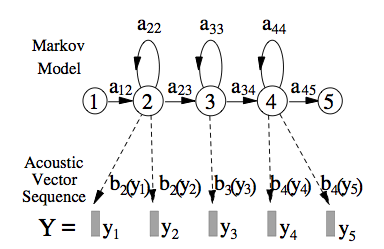
\includegraphics[width=0.5\textwidth]{figures/asr_hmm.png}
            \caption{A HMM as it is commonly used in ASR, with phonemes as hidden states and acoustic feature vectors as the observations. $a_12, a_22, a_23,...$ are elements of the transition matrix $A$; $b_2(y1_), b_2(y_2), b_3(y_3)$ are elements of the output probability matrix $B$; $Y = y_1,y_2,...$ is the observation sequence. \cite{gales_young_hmm}}
            \label{fig:asr_hmm}
        \end{center}
    \end{figure}